\documentclass{report}\usepackage[]{graphicx}\usepackage[]{color}
%% maxwidth is the original width if it is less than linewidth
%% otherwise use linewidth (to make sure the graphics do not exceed the margin)
\makeatletter
\def\maxwidth{ %
  \ifdim\Gin@nat@width>\linewidth
    \linewidth
  \else
    \Gin@nat@width
  \fi
}
\makeatother

\definecolor{fgcolor}{rgb}{0.345, 0.345, 0.345}
\newcommand{\hlnum}[1]{\textcolor[rgb]{0.686,0.059,0.569}{#1}}%
\newcommand{\hlstr}[1]{\textcolor[rgb]{0.192,0.494,0.8}{#1}}%
\newcommand{\hlcom}[1]{\textcolor[rgb]{0.678,0.584,0.686}{\textit{#1}}}%
\newcommand{\hlopt}[1]{\textcolor[rgb]{0,0,0}{#1}}%
\newcommand{\hlstd}[1]{\textcolor[rgb]{0.345,0.345,0.345}{#1}}%
\newcommand{\hlkwa}[1]{\textcolor[rgb]{0.161,0.373,0.58}{\textbf{#1}}}%
\newcommand{\hlkwb}[1]{\textcolor[rgb]{0.69,0.353,0.396}{#1}}%
\newcommand{\hlkwc}[1]{\textcolor[rgb]{0.333,0.667,0.333}{#1}}%
\newcommand{\hlkwd}[1]{\textcolor[rgb]{0.737,0.353,0.396}{\textbf{#1}}}%
\let\hlipl\hlkwb

\usepackage{framed}
\makeatletter
\newenvironment{kframe}{%
 \def\at@end@of@kframe{}%
 \ifinner\ifhmode%
  \def\at@end@of@kframe{\end{minipage}}%
  \begin{minipage}{\columnwidth}%
 \fi\fi%
 \def\FrameCommand##1{\hskip\@totalleftmargin \hskip-\fboxsep
 \colorbox{shadecolor}{##1}\hskip-\fboxsep
     % There is no \\@totalrightmargin, so:
     \hskip-\linewidth \hskip-\@totalleftmargin \hskip\columnwidth}%
 \MakeFramed {\advance\hsize-\width
   \@totalleftmargin\z@ \linewidth\hsize
   \@setminipage}}%
 {\par\unskip\endMakeFramed%
 \at@end@of@kframe}
\makeatother

\definecolor{shadecolor}{rgb}{.97, .97, .97}
\definecolor{messagecolor}{rgb}{0, 0, 0}
\definecolor{warningcolor}{rgb}{1, 0, 1}
\definecolor{errorcolor}{rgb}{1, 0, 0}
\newenvironment{knitrout}{}{} % an empty environment to be redefined in TeX

\usepackage{alltt}

\usepackage{polyglossia}
  \setmainlanguage{spanish}
\usepackage{fontspec}
\usepackage{geometry}
\usepackage{parskip}
\usepackage{amsmath}
\usepackage{subcaption}
\usepackage{pgfplots}
  \pgfplotsset{compat=1.12}
  \makeatletter
    \pgfdeclareplotmark{dot}
      {%
        \fill circle [x radius=0.04, y radius=0.16];
      }%
  \makeatother
\usepackage{booktabs}
\usepackage{makeidx}
  \makeindex
\usepackage[backend=bibtex,style=authoryear,citestyle=authoryear,doi=false,isbn=false,url=false]{biblatex}
  \addbibresource{NER-bib.bib}
\usepackage[hidelinks,spanish]{hyperref}

%pgfplot función normal
\pgfmathdeclarefunction{gauss}{2}{%
  \pgfmathparse{1/(#2*sqrt(2*pi))*exp(-((x-#1)^2)/(2*#2^2))}%
}

\newcommand*{\eng}[1]{\textsl{#1}}
\newcommand*{\paq}[1]{\textbf{#1}\index{#1@\textbf{#1}}}
\newcommand*{\kw}[1]{\textbf{#1}\index{#1}}

\newcommand{\Var}{\operatorname{Var}}
\newcommand{\Cov}{\operatorname{Cov}}
\newcommand{\E}{\operatorname{E}}
\newcommand{\sd}{\operatorname{de}}
\newcommand{\se}{\operatorname{se}}

% Eliminar numeración en títulos menores que secciones
\setcounter{secnumdepth}{2}

% Code chunk



\title{Notas de Econometría en R}
\author{Alvaro Carril\thanks{Estas notas son un intento de condensar lo justo y necesario para poder seguir un curso de econometría con R.
Luego de recopilar material de muchas clases y ayudantías de econometría, en general pensadas para ser aplicadas en Stata, decidí que podía intentar hacer estas clases en R y usar esta guía como material de apoyo.
Mi prioridad fue ser breve y conciso, por lo que estas notas no son un buen comienzo para aprender R (o econometría); son un complemento.
Si hay algún error o quieres hacer algún comentario, mi correo es \texttt{acarril@fen.uchile.cl}.}}
\IfFileExists{upquote.sty}{\usepackage{upquote}}{}
\begin{document}

\maketitle
\tableofcontents

\clearpage

% Introducción, prefacio:



\chapter{Introducción}

En las últimas décadas la economía se ha ido apropiando de los computadores para realizar trabajo empírico y, sin embargo, el enfoque de los libros de econometría sigue siendo eminentemente teórico ---no \emph{aplicado}.

A mi parecer, existen actualmente dos maneras de abordar la enseñanza de econometría. La primera es la clásica, o \emph{matemática}: derivando los modelos desde como ejercicios de álgebra lineal, y en general priorizando aspectos técnicos por sobre los conceptuales o aplicados. Vemos esto en libros que discuten en extensión los supuestos detrás de las formas funcionales o supuestos de distribución, pero que dedican pocas palabras a técnicas aplicadas como métodos de regresión discontinua.

Por otro lado hay quienes, de la mano con el crecimiento de la economía aplicada, abogan por una enseñanza aplicada de econometría, con énfasis en técnicas de 

\section{Qué es R}

R es un ambiente de software y un lenguaje de programación interpretado para hacer análisis estadístico y crear gráficos. Es una implementación de S, un lenguaje de programación matemático orientado a objetos más antiguo. Es software libre y de código abierto, constantemente desarrollado por estadísticos y colaboradores de otras disciplinas.

R es mucho más flexible que la mayoría de los paquetes estadísticos normalmente usados por economistas. Es un lenguaje de programación completamente desarrollado, no sólo un programa con tests y métodos pre-programados.


\section{Obtener R}

La instalación base de R puede obtenerse de \url{https://www.r-project.org/}. Una vez instalado puedes usar RGui para usarlo. Sin embargo, usualmente yo tomo dos pasos adicionales para obtener más flexibilidad. El primero es instalar RStudio, un IDE para R que incluye una consola, editor con resaltado de sintaxis, historial de comandos y varias otras vainas que lo hacen más útil que RGui, especialmente si eres principiante. Puedes descargar RStudio de \url{https://www.rstudio.com/}, y también es gratis.

Finalmente, a mi me gusta poder interactuar con R desde la línea de comandos, igual que puedo hacer con Python o Julia. Para poder hacer esto en Windows tenemos que ejecutar R:

\begin{knitrout}
\definecolor{shadecolor}{rgb}{0.969, 0.969, 0.969}\color{fgcolor}\begin{kframe}
\begin{alltt}
\hlstr{"C:\textbackslash{}Program Files\textbackslash{}R\textbackslash{}R-3.4.0\textbackslash{}bin\textbackslash{}x64\textbackslash{}R"}
\end{alltt}
\end{kframe}
\end{knitrout}

Obviamente, tienes que reemplazar este directorio por el que corresponde a tu instalación. 

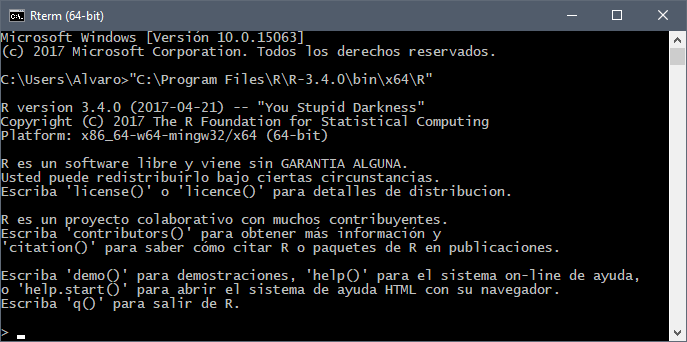
\includegraphics[width=\linewidth]{sss/r-win-command-prompt}

\subsection{Usar R interactivamente y a través de scripts}

\begin{knitrout}
\definecolor{shadecolor}{rgb}{0.969, 0.969, 0.969}\color{fgcolor}\begin{kframe}
\begin{alltt}
\hlkwd{getwd}\hlstd{()}
\end{alltt}
\begin{verbatim}
## [1] "/Users/alvaro/Dropbox (Personal)/Proyectos/NER"
\end{verbatim}
\end{kframe}
\end{knitrout}



\section{Trabajando con datos}

\subsection{Objetos y asignaciones}

R es un lenguaje interpretado, lo que significa que ejecuta nuestras instrucciones directamente, sin compilar un programa previo. Podemos usar R interactivamente a través de la consola:
\begin{knitrout}
\definecolor{shadecolor}{rgb}{0.969, 0.969, 0.969}\color{fgcolor}\begin{kframe}
\begin{alltt}
\hlnum{1}\hlopt{+}\hlnum{2}
\end{alltt}
\begin{verbatim}
## [1] 3
\end{verbatim}
\end{kframe}
\end{knitrout}

La mayoría de las operaciones y funciones en R no guardan el resultado de su ejecución. Por ejemplo, el resultado anterior (\verb|3|) es calculado pero no puede ser reutilizado sin volverse a calcular. Para lograr esto tenemos que asignar el resultado de la operación a un objeto:
\begin{knitrout}
\definecolor{shadecolor}{rgb}{0.969, 0.969, 0.969}\color{fgcolor}\begin{kframe}
\begin{alltt}
\hlstd{x} \hlkwb{<-} \hlnum{1}\hlopt{+}\hlnum{2}
\end{alltt}
\end{kframe}
\end{knitrout}


% Introducción, prefacio:



\chapter{Regresión lineal}



El modelo de regresión lineal es el caballo de batalla de la econometría aplicada.
En su forma más simple usualmente se escribe como
\begin{equation}
y_i = \beta_0 + \beta_1 x_i + \mu_i.
\label{eq:modelo_lineal_simple}
\end{equation}
donde $i = 1, \ldots, n$ es un índice que identifica a las observaciones (filas) en los datos. Podríamos tener $n$ personas, familias o empresas. Los términos $x$ e $y$ son vectores de datos de tamaño $n$.

En este modelo suponemos que la variable dependiente $y$ es una función lineal de la variable independiente, $x$. Entonces intentaremos buscar ---o \emph{estimar}--- una combinación de parámetros $\beta_0$ y $\beta_1$ que se ajuste a nuestros datos. Como es posible que los datos no tengan una relación lineal perfecta, el modelo incluye un término de error $\mu_i$. Este término representa otras variables que afectan a $y_i$ que no sean $x_i$.

Por ejemplo, podríamos tener un vector $y$ con los salarios de $n$ personas y modelarlo como una función lineal de los años de educación de esas personas, $x$. Resulta útil tener una base de datos concreta con estos vectores, por lo que usaremos 

\begin{knitrout}
\definecolor{shadecolor}{rgb}{0.969, 0.969, 0.969}\color{fgcolor}\begin{kframe}
\begin{alltt}
\hlcom{#simdatos <- read.csv(}
\hlcom{#  "https://raw.githubusercontent.com/acarril/NER/master/datos/simdatos.csv")}
\hlstd{simdatos} \hlkwb{<-} \hlkwd{read.csv}\hlstd{(}\hlstr{"datos/simdatos.csv"}\hlstd{)}
\hlkwd{head}\hlstd{(simdatos)}
\end{alltt}
\begin{verbatim}
##   y         x
## 1 1  4.199913
## 2 1  7.510634
## 3 1  2.125473
## 4 2  8.988857
## 5 2 10.243105
## 6 2 11.296823
\end{verbatim}
\end{kframe}
\end{knitrout}

El comando \verb|read.csv()| permite leer bases de datos en formato CSV. Lo usamos para leer una base en línea y luego asignamos esos datos al objeto \verb|simdatos| (datos simulados). 
La función \verb|head()| sirve para imprimir el encabezado de los datos, lo que permite hacernos una idea rápida de las variables y sus valores.
Esta base tiene 30 observaciones (puedes imprimirla completa ejecutado \verb|simdatos|). La variable \verb|y| representa ingreso por hora (en miles de pesos) y la variable \verb|x| representa años de educación.

Siempre es recomendable graficar los datos, ya que un gráfico entrega mucha información y revela patrones. Para esto usaremos \paq{ggplot2}, un paquete muy poderoso para crear gráficos de distintos tipos. Lo cargamos y luego creamos un gráfico de puntos con los datos:

\begin{knitrout}
\definecolor{shadecolor}{rgb}{0.969, 0.969, 0.969}\color{fgcolor}\begin{kframe}
\begin{alltt}
\hlkwd{library}\hlstd{(ggplot2)}
\hlkwd{ggplot}\hlstd{(simdatos,} \hlkwd{aes}\hlstd{(x, y))} \hlopt{+} \hlkwd{geom_point}\hlstd{()}
\end{alltt}
\end{kframe}

{\centering \includegraphics[width=4in,height=3in]{figs/unnamed-chunk-7-1} 

}



\end{knitrout}

Vemos que existe una evidente relación lineal entre $x$ e $y$: a mayor nivel de educación parece haber mayor nivel de ingreso.
Esto es bueno para nosotros, ya que queremos ajustar los datos a un modelo lineal como el que escribimos en \eqref{eq:modelo_lineal_simple}.
Cabe preguntarse ahora cuál es la manera óptima de elegir los parámetros que determinan dicha relación lineal, es decir, ¿cómo podemos elegir $\beta_0$ (el intercepto) y $\beta_1$ (la pendiente) para que la predicción se ajuste lo mejor posible a los datos?

Podríamos elegir entre una infinita variedad de combinaciones de $\beta_0$ y $\beta_1$ para modelar los datos. Por ejemplo, el código de abajo simula 150 líneas con interceptos y pendientes ``razonables'':

\begin{knitrout}
\definecolor{shadecolor}{rgb}{0.969, 0.969, 0.969}\color{fgcolor}\begin{kframe}
\begin{alltt}
\hlkwd{set.seed}\hlstd{(}\hlnum{314}\hlstd{)}
\hlstd{modelos} \hlkwb{<-} \hlkwd{data.frame}\hlstd{(}
  \hlkwc{beta1} \hlstd{=} \hlkwd{runif}\hlstd{(}\hlnum{150}\hlstd{,} \hlopt{-}\hlnum{3}\hlstd{,} \hlnum{1}\hlstd{),}
  \hlkwc{beta2} \hlstd{=} \hlkwd{runif}\hlstd{(}\hlnum{150}\hlstd{,} \hlopt{-}\hlnum{1}\hlstd{,} \hlnum{1}\hlstd{)}
\hlstd{)}
\hlkwd{ggplot}\hlstd{(simdatos,} \hlkwd{aes}\hlstd{(x, y))} \hlopt{+}
  \hlkwd{geom_point}\hlstd{()} \hlopt{+}
  \hlkwd{geom_abline}\hlstd{(}
    \hlkwd{aes}\hlstd{(}\hlkwc{intercept} \hlstd{= beta1,} \hlkwc{slope} \hlstd{= beta2),}
    \hlkwc{data} \hlstd{= modelos,} \hlkwc{alpha} \hlstd{=} \hlnum{1}\hlopt{/}\hlnum{4}
  \hlstd{)}
\end{alltt}
\end{kframe}

{\centering \includegraphics[width=4in,height=3in]{figs/unnamed-chunk-8-1} 

}



\end{knitrout}

Si bien hay muchas líneas que claramente no se ajustan bien a los datos, varias otras sí lo hacen, y resulta difícil determinar cuál es ``la mejor'' (asumiendo que tal línea existe).
Necesitamos un criterio riguroso para elegir los parámetros $\beta_0$ y $\beta_1$ de manera óptima, y esto es lo que haremos a continuación.


\subsection{Mínimos Cuadrados Ordinarios}
\label{sec:MCO}

El método de Mínimos Cuadrados Ordinarios (MCO) es una respuesta directa a la pregunta que planteamos recién: ¿qué criterio conviene usar para elegir el modelo lineal que se ajuste ``mejor'' a los datos?
Geométricamente, el método de MCO equivale a minimizar la distancia vertical entre los puntos y la recta definida por el modelo.

\begin{knitrout}
\definecolor{shadecolor}{rgb}{0.969, 0.969, 0.969}\color{fgcolor}

{\centering \includegraphics[width=4in,height=3in]{figs/unnamed-chunk-9-1} 

}



\end{knitrout}

Recordemos que nuestro modelo original es
\begin{equation*}
y_i = \beta_0 + \beta_1 x_i + \mu_i.
\end{equation*}
Dada una muestra de datos (como \verb|simdatos|), llamamos $\hat\beta_0$ y $\hat\beta_1$ a los candidatos para los coeficientes de la estimación. Entonces la recta $y_i$ que estimamos está definida como
\begin{equation}
\hat y_i = \hat\beta_0 + \hat\beta_1 x_i.
\end{equation}

La diferencia entre $y_i$ (los datos) y $\hat y_i$ (nuestra predicción) corresponde a $\hat\mu_i$, el residuo de nuestra estimación para cada observación $i$: 
\begin{align}
\hat \mu_i &= y_i - \hat y_i \notag \\
           &= y_i - \hat\beta_0 + \hat\beta_1 x_i.
\label{eq:residuos}
\end{align}
Gráficamente, la distancia entre cada punto (los datos) y la recta (la predicción $\hat y_i$)  corresponde al residuo, $\hat\mu_i$, representada en el gráfico por las líneas rojas. 
Es decir que para cada observación $i$ tenemos una medida de la magnitud del error que esta elección de $\hat\beta_0$ y $\hat\beta_1$ produce.
El método de MCO corresponde a elegir $\hat\beta_0$ y $\hat\beta_1$ en \eqref{eq:residuos} tal que se minimice la suma de los residuos al cuadrado:\footnote{¿Por qué al cuadrado? Porque se asume que es irrelevante si el error es una subestimación o una sobreestimación, de forma que lo único que importa es la magnitud. ¿Por qué no se usa el valor absoluto entonces? Buena pregunta: \url{https://stats.stackexchange.com/q/46019/91358}. Básicamente, porque es algebraicamente más simple manejar valores al cuadrado, y no hace ninguna diferencia en el resultado final.}

\begin{align}
\min_{\hat\beta_0,\hat\beta_1} & \sum_{i=1}^n \hat\mu_i^2 \notag \\
\Leftrightarrow \min_{\hat\beta_0,\hat\beta_1} & \sum_{i=1}^n (y_i - \hat\beta_0 - \hat\beta_1 x_i)^2.
\label{eq:prob_min_MCO}
\end{align}

Al resolver este problema de minimización obtendremos los estimadores MCO:\footnote{La derivación paso a paso puede encontrarse, por ejemplo, en \textcite[cap. 2]{wooldridge_introductory_2013}.}

\begin{align}
\hat \beta_1 &= \sum_{i=1}^n \frac{\sum_{i=1}^n (x_i - \bar x)(y_i - \bar y)}{\sum_{i=1}^n (x_i - \bar x)^2} \notag \\
 &= \frac{\Cov (x,y)}{\Var(x)} \\
\hat \beta_0 &= \bar y - \hat\beta_1 \bar x
\end{align}
donde $\bar x$ e $\bar y$ son los promedios de $x_i$ e $y_i$, $\Var(x)$ es la varianza muestral de $x$ y $\Cov(x,y)$ es la covarianza muestral de $x$ e $y$.
Todo esto significa que para encontrar los estimadores MCO y obtener la línea de mejor ajuste simplemente tenemos que calcular cuatro cosas: $\bar y$, $\bar x$, $\Cov (x,y)$ y $\Var (x,y)$. ¡Hagámoslo ahora!

\begin{knitrout}
\definecolor{shadecolor}{rgb}{0.969, 0.969, 0.969}\color{fgcolor}\begin{kframe}
\begin{alltt}
\hlcom{# Indicar base de datos a usar}
\hlkwd{attach}\hlstd{(simdatos)}
\hlcom{# Promedios de 'x' e 'y'}
\hlstd{x.barra} \hlkwb{<-} \hlkwd{mean}\hlstd{(x)}
\hlstd{y.barra} \hlkwb{<-} \hlkwd{mean}\hlstd{(y)}
\hlcom{# Varianza de 'x' y covarianza entre 'x' e 'y'}
\hlstd{var.x} \hlkwb{<-} \hlkwd{var}\hlstd{(x)}
\hlstd{cov.xy} \hlkwb{<-} \hlkwd{cov}\hlstd{(x,y)}
\hlcom{# Calcular parámetros MCO}
\hlstd{beta1} \hlkwb{<-} \hlstd{cov.xy}\hlopt{/}\hlstd{var.x}
\hlstd{beta0} \hlkwb{<-} \hlstd{y.barra} \hlopt{-} \hlstd{beta1}\hlopt{*}\hlstd{x.barra}
\hlcom{# 'Desactivar' base de datos}
\hlkwd{detach}\hlstd{(simdatos)}
\hlcom{# Imprimir parámetros calculados}
\hlstd{beta0}
\end{alltt}
\begin{verbatim}
## [1] -1.185369
\end{verbatim}
\begin{alltt}
\hlstd{beta1}
\end{alltt}
\begin{verbatim}
## [1] 0.4311958
\end{verbatim}
\end{kframe}
\end{knitrout}
Vemos que es fácil calcular los estimadores MCO y en este caso $\hat \beta_0 = -1.19$ y $\hat \beta_1 = 0.43$.

Ahora podemos usar los parámetros estimados para graficar $\hat y_i$ sobre los datos:

\begin{knitrout}
\definecolor{shadecolor}{rgb}{0.969, 0.969, 0.969}\color{fgcolor}\begin{kframe}
\begin{alltt}
\hlcom{# Graficar línea de regresión MCO}
\hlkwd{ggplot}\hlstd{(simdatos,} \hlkwd{aes}\hlstd{(x,y))} \hlopt{+}
  \hlkwd{expand_limits}\hlstd{(}\hlkwc{x} \hlstd{=} \hlnum{0}\hlstd{,} \hlkwc{y} \hlstd{=} \hlopt{-}\hlnum{2.5}\hlstd{)} \hlopt{+}
  \hlkwd{geom_point}\hlstd{()} \hlopt{+}
  \hlkwd{geom_abline}\hlstd{(}
    \hlkwc{intercept} \hlstd{= beta0,} \hlkwc{slope} \hlstd{= beta1,}
    \hlkwc{color} \hlstd{=} \hlstr{"blue"}\hlstd{,} \hlkwc{show.legend} \hlstd{=} \hlnum{FALSE} \hlstd{)}
\end{alltt}
\end{kframe}

{\centering \includegraphics[width=4in,height=3in]{figs/unnamed-chunk-11-1} 

}



\end{knitrout}

Si bien el método que acabamos de usar para calcular $\hat\beta_0$ y $\hat\beta_1$ es útil para entender de manera más profunda qué es lo que estamos haciendo al estimar un modelo líneal por el método de MCO, no es demasiado breve. Podemos obtener los parámetros directamente usando la función \verb|lm()| de la siguiente forma:

\begin{knitrout}
\definecolor{shadecolor}{rgb}{0.969, 0.969, 0.969}\color{fgcolor}\begin{kframe}
\begin{alltt}
\hlkwd{lm}\hlstd{(y} \hlopt{~} \hlstd{x,} \hlkwc{data} \hlstd{= simdatos)}
\end{alltt}
\begin{verbatim}
## 
## Call:
## lm(formula = y ~ x, data = simdatos)
## 
## Coefficients:
## (Intercept)            x  
##     -1.1854       0.4312
\end{verbatim}
\end{kframe}
\end{knitrout}

La función \verb|lm()| viene de \eng{linear model}, y permite calcular rápidamente los parámetros de un modelo lineal (¡usamos una línea!). El primer argumento de la función es una fórmula de R, que no es exactamente lo mismo que una fórmula en el sentido usual de la palabra. Por el momento basta entender que a la izquierda de \verb|~| indicamos la variable dependiente, mientras que a la derecha indicamos las variables independientes. Entonces \verb|lm()| toma una fórmula como \verb|y~x| y la traduce automáticamente a algo como \verb|y = beta0 + beta1 * x|.

Una de las ventajas de usar \verb|lm()| es que podemos guardar sus resultados en un objeto, el que luego podemos manipular para extraer otro tipo de información útil del modelo. A continuación veremos cómo extraer, manipular e interpretar esta información, lo que nos dará una comprensión mucho más profunda de lo que estamos haciendo.


\subsection{Interpretando un modelo lineal}

Usaremos ahora la base \verb|wage2|, que es uno de los datos usados por \textcite{wooldridge_introductory_2013} y contiene información de ingresos (y otras variables) para 935 personas. \footnote{Esta base es un subconjunto de los datos del estudio de \textcite{blackburn_unobserved_1992}.}

\begin{knitrout}
\definecolor{shadecolor}{rgb}{0.969, 0.969, 0.969}\color{fgcolor}\begin{kframe}
\begin{alltt}
\hlkwd{library}\hlstd{(foreign)}
\hlcom{#ingresos <- read.dta("http://fmwww.bc.edu/ec-p/data/wooldridge/wage2.dta")}
\hlstd{ingresos} \hlkwb{<-} \hlkwd{read.dta}\hlstd{(}\hlstr{"datos/wage2.dta"}\hlstd{)}
\hlstd{ingresos} \hlkwb{<-} \hlkwd{as.data.frame}\hlstd{(ingresos[}\hlkwd{c}\hlstd{(}\hlstr{"wage"}\hlstd{,}\hlstr{"educ"}\hlstd{)])}
\end{alltt}
\end{kframe}
\end{knitrout}

El paquete \paq{foreign} nos permite leer bases de datos en formatos de otros programas. En este caso usamos la función \verb|foreign::read.dta()| para leer una base de datos de Stata.
Por el momento nos interesan dos variables: \verb|wage|, que es un vector de ingresos (en dólares menusales) y \verb|educ|, que es un vector con años de escolaridad de cada persona. La última línea guarda solamente esas dos variables, como marco de datos, en el objeto \verb|ingresos|.

Al cargar nuevos datos yo siempre recomiendo:
\begin{enumerate}
\item Imprimir el encabezado
\item Imprimir un resumen
\item Graficarlos
\end{enumerate}

Escribimos lo siguiente para lograr estas tres cosas:

\begin{knitrout}
\definecolor{shadecolor}{rgb}{0.969, 0.969, 0.969}\color{fgcolor}\begin{kframe}
\begin{alltt}
\hlkwd{head}\hlstd{(ingresos)}
\end{alltt}
\begin{verbatim}
##   wage educ
## 1  769   12
## 2  808   18
## 3  825   14
## 4  650   12
## 5  562   11
## 6 1400   16
\end{verbatim}
\begin{alltt}
\hlkwd{summary}\hlstd{(ingresos)}
\end{alltt}
\begin{verbatim}
##       wage             educ      
##  Min.   : 115.0   Min.   : 9.00  
##  1st Qu.: 669.0   1st Qu.:12.00  
##  Median : 905.0   Median :12.00  
##  Mean   : 957.9   Mean   :13.47  
##  3rd Qu.:1160.0   3rd Qu.:16.00  
##  Max.   :3078.0   Max.   :18.00
\end{verbatim}
\begin{alltt}
\hlkwd{ggplot}\hlstd{(ingresos,} \hlkwd{aes}\hlstd{(educ, wage))} \hlopt{+} \hlkwd{geom_point}\hlstd{()}
\end{alltt}
\end{kframe}

{\centering \includegraphics[width=4in,height=3in]{figs/unnamed-chunk-14-1} 

}



\end{knitrout}

Es evidente que estos datos (reales) no presentan una relación lineal tan evidente. Más adelante nos haremos cargo de este problema.

\subsubsection{Coeficientes}

Volvemos a usar \verb|lm()| como ya lo hemos hecho, esta vez definiendo una fórmula donde \verb|wage| es la variable dependiente y \verb|educ| es la variable independiente:
\begin{knitrout}
\definecolor{shadecolor}{rgb}{0.969, 0.969, 0.969}\color{fgcolor}\begin{kframe}
\begin{alltt}
\hlkwd{lm}\hlstd{(wage} \hlopt{~} \hlstd{educ,} \hlkwc{data} \hlstd{= ingresos)}
\end{alltt}
\begin{verbatim}
## 
## Call:
## lm(formula = wage ~ educ, data = ingresos)
## 
## Coefficients:
## (Intercept)         educ  
##      146.95        60.21
\end{verbatim}
\end{kframe}
\end{knitrout}


Los coeficientes estimados de un modelo lineal como este pueden interpretarse fácilmente, recordando que nuestra predicción es
\begin{equation*}
\hat y = \hat \beta_0 + \hat \beta_1 x.
\end{equation*}
Notar que esta ecuación es equivalente a una función lineal genérica, del tipo $y=a+bx$. Tener este simple hecho en cuenta es de gran ayuda para entender su interpretación.

El intercepto de un modelo lineal nos indica que si las variables independientes son todas iguales a 0, el modelo predice, en promedio, un valor de $\hat \beta_0$ para $\hat y$. En este ejemplo, si una persona tiene 0 años de educación el modelo predice un ingreso mensual promedio de 146.95 dólares.
Los coeficientes estimados para las variables independientes (solamente $\hat \beta_1$, en este caso) pueden interpretarse como el cambio promedio que un aumento de una unidad de $x$ tiene sobre $y$. Nuestra estimación indica que un año adicional de educación tiene un efecto promedio de aumentar en 60.21 dólares el ingreso de las personas. Si este coeficiente fuera negativo diríamos que un cambio en $x$ está correlacionado a una reducción de $y$.


\subsubsection{Errores estándar de los coeficientes}

Los parámetros estimados ---los coeficientes de MCO, en este caso--- son estadísticos muestrales que usamos para hacer inferencias de los parámetros poblacionales. Es importante tener en cuenta que son estos parámetros poblacionales los que nos interesan en realidad, pero como no podemos observarlos directamente, debemos inferirlos por medio de una muestra finita.

Es evidente que si tomáramos una muestra distinta a la actual, lo más probable es que estimaríamos parámetros diferentes. Si tomaras datos de otras 935 personas (o cualquier número, en realidad) es muy posible que al aplicar el mismo modelo obtuviéramos valores de $\beta_0$ y $\beta_1$ distintos de 146.95 y 60.21. Además es muy probable que nuevamente ninguno de los dos sea igual al verdadero parámetro poblacional, que es el que nos interesa. Si continuáramos este proceso de tomar diferentes muestras y estimar los mismos parámetros una y otra vez, veríamos que la frecuencia relativa de las estimaciones obtenidas sigue una distribución de probabilidad, y por el Teorema Central del Límite sabemos que es probable que esta distribución sea normal. Entonces es importante para nuestra estimación que cuantifiquemos la cantidad de incertidumbre en esta distribución poblacional desconocida. Ahí es donde entra el concepto de error estándar, que corresponde a nuestra estimación de la desviación estándar de la distribución de estos muestreos. En términos intuitivos, es una medida de la incertidumbre de $\hat\beta$.

Encerramos \verb|lm()| dentro de \verb|summary()| para obtener información más detallada de las estimaciones del modelo, incluyendo estimaciones para los errores estándar de los coeficientes:

\begin{knitrout}
\definecolor{shadecolor}{rgb}{0.969, 0.969, 0.969}\color{fgcolor}\begin{kframe}
\begin{alltt}
\hlkwd{summary}\hlstd{(}\hlkwd{lm}\hlstd{(wage} \hlopt{~} \hlstd{educ,} \hlkwc{data} \hlstd{= ingresos))}
\end{alltt}
\begin{verbatim}
## 
## Call:
## lm(formula = wage ~ educ, data = ingresos)
## 
## Residuals:
##    Min     1Q Median     3Q    Max 
## -877.4 -268.6  -38.4  207.0 2148.3 
## 
## Coefficients:
##             Estimate Std. Error t value Pr(>|t|)    
## (Intercept)   146.95      77.71    1.89    0.059 .  
## educ           60.21       5.69   10.57   <2e-16 ***
## ---
## Signif. codes:  0 '***' 0.001 '**' 0.01 '*' 0.05 '.' 0.1 ' ' 1
## 
## Residual standard error: 382 on 933 degrees of freedom
## Multiple R-squared:  0.107,	Adjusted R-squared:  0.106 
## F-statistic:  112 on 1 and 933 DF,  p-value: <2e-16
\end{verbatim}
\end{kframe}
\end{knitrout}

En el ejemplo, ...

%todo: explicar mejor todos los summary de ols

\begin{knitrout}
\definecolor{shadecolor}{rgb}{0.969, 0.969, 0.969}\color{fgcolor}\begin{kframe}
\begin{alltt}
\hlkwd{ggplot}\hlstd{(ingresos,} \hlkwd{aes}\hlstd{(educ, wage))} \hlopt{+}
  \hlkwd{geom_point}\hlstd{()} \hlopt{+}
  \hlkwd{geom_smooth}\hlstd{(}\hlkwc{method} \hlstd{=} \hlstr{"lm"}\hlstd{)}
\end{alltt}
\end{kframe}

{\centering \includegraphics[width=4in,height=3in]{figs/unnamed-chunk-18-1} 

}



\end{knitrout}


\subsection{Extraer estadísticos de una regresión}

Para guardar el modelo asignamos \verb|lm()| a un objeto:

\begin{knitrout}
\definecolor{shadecolor}{rgb}{0.969, 0.969, 0.969}\color{fgcolor}\begin{kframe}
\begin{alltt}
\hlstd{modelo} \hlkwb{<-} \hlkwd{lm}\hlstd{(wage} \hlopt{~} \hlstd{educ,} \hlkwc{data} \hlstd{= ingresos)}
\end{alltt}
\end{kframe}
\end{knitrout}

El objeto \verb|modelo| no solo incluye los coeficientes estimados, si no que una serie de otros elementos que son muy útiles ---veremos ahora por qué. En estricto rigor \verb|modelo| es lo que R llama una lista, y contiene una serie de otros objetos. Podemos imprimir los nombres de estos objetos escribiendo
\begin{knitrout}
\definecolor{shadecolor}{rgb}{0.969, 0.969, 0.969}\color{fgcolor}\begin{kframe}
\begin{alltt}
\hlkwd{names}\hlstd{(modelo)}
\end{alltt}
\begin{verbatim}
##  [1] "coefficients"  "residuals"     "effects"       "rank"         
##  [5] "fitted.values" "assign"        "qr"            "df.residual"  
##  [9] "xlevels"       "call"          "terms"         "model"
\end{verbatim}
\end{kframe}
\end{knitrout}

Para acceder a los objetos guardados usamos la notación de \verb|$|, como es usual en R. Por ejemplo, para imprimir los coeficientes del modelo escribimos
\begin{knitrout}
\definecolor{shadecolor}{rgb}{0.969, 0.969, 0.969}\color{fgcolor}\begin{kframe}
\begin{alltt}
\hlstd{modelo}\hlopt{$}\hlstd{coefficients}
\end{alltt}
\begin{verbatim}
## (Intercept)        educ 
##         147          60
\end{verbatim}
\end{kframe}
\end{knitrout}
También existen funciones para acceder directamente a los objetos. Por ejemplo,
\begin{knitrout}
\definecolor{shadecolor}{rgb}{0.969, 0.969, 0.969}\color{fgcolor}\begin{kframe}
\begin{alltt}
\hlkwd{coefficients}\hlstd{(modelo)}
\end{alltt}
\begin{verbatim}
## (Intercept)        educ 
##         147          60
\end{verbatim}
\end{kframe}
\end{knitrout}
En cualquier caso, el resultado es un vector cuyos elementos tienen nombres: el intercepto ($\beta_0$) es \texttt{(Intercept)} y el nombre del primer coeficiente ($\beta_1$) es el nombre de la variable $x$, es decir, \texttt{educ}. Usando esto podemos acceder a elementos específicos del vector usando sus nombres o sus índices, como se mencionó en [ref]:
\begin{knitrout}
\definecolor{shadecolor}{rgb}{0.969, 0.969, 0.969}\color{fgcolor}\begin{kframe}
\begin{alltt}
\hlkwd{coef}\hlstd{(modelo)[}\hlnum{1}\hlstd{]}
\end{alltt}
\begin{verbatim}
## (Intercept) 
##         147
\end{verbatim}
\begin{alltt}
\hlkwd{coef}\hlstd{(modelo)[}\hlstr{"educ"}\hlstd{]}
\end{alltt}
\begin{verbatim}
## educ 
##   60
\end{verbatim}
\end{kframe}
\end{knitrout}

\subsection{Predicciones y residuos}

La predicción de un modelo, a veces llamada valores ajustados, es simplemente el vector $\hat y_i$. Teniendo los valores ajustados podemos calcular también los residuos del modelo, $\mu_i$:
\begin{align}
\hat y_i &= \hat \beta_0 + \hat\beta_1 x_i \label{eq:prediccion} \\
\hat \mu_i &= y_i - \hat y_i \label{eq:residuos}
\end{align}
Podemos calcular fácilmente ambos vectores con los elementos que tenemos:
\begin{knitrout}
\definecolor{shadecolor}{rgb}{0.969, 0.969, 0.969}\color{fgcolor}\begin{kframe}
\begin{alltt}
\hlstd{ingresos}\hlopt{$}\hlstd{prediccion} \hlkwb{<-} \hlkwd{coef}\hlstd{(modelo)[}\hlnum{1}\hlstd{]} \hlopt{+} \hlkwd{coef}\hlstd{(modelo)[}\hlnum{2}\hlstd{]} \hlopt{*} \hlstd{ingresos}\hlopt{$}\hlstd{educ}
\hlstd{ingresos}\hlopt{$}\hlstd{residuos} \hlkwb{<-} \hlstd{ingresos}\hlopt{$}\hlstd{wage} \hlopt{-} \hlstd{ingresos}\hlopt{$}\hlstd{prediccion}
\end{alltt}
\end{kframe}
\end{knitrout}

Alternativamente, podemos calcular los valores predichos y los residuos del modelo usando funciones específicas para ello:
\begin{knitrout}
\definecolor{shadecolor}{rgb}{0.969, 0.969, 0.969}\color{fgcolor}\begin{kframe}
\begin{alltt}
\hlstd{modelo.sim} \hlkwb{<-} \hlkwd{lm}\hlstd{(y} \hlopt{~} \hlstd{x,} \hlkwc{data} \hlstd{= simdatos)}
\hlstd{simdatos}\hlopt{$}\hlstd{prediccion} \hlkwb{<-} \hlkwd{fitted}\hlstd{(modelo.sim)}
\hlstd{simdatos}\hlopt{$}\hlstd{residuos} \hlkwb{<-} \hlkwd{resid}\hlstd{(modelo.sim)}
\end{alltt}
\end{kframe}
\end{knitrout}

Podemos graficar nuestra predicción sobre los datos para inspeccionar visualmente cómo se ve. Para esto volvemos a usar \paq{ggplot2}:
\begin{knitrout}
\definecolor{shadecolor}{rgb}{0.969, 0.969, 0.969}\color{fgcolor}\begin{kframe}
\begin{alltt}
\hlkwd{ggplot}\hlstd{(ingresos,} \hlkwd{aes}\hlstd{(educ, wage))} \hlopt{+}
  \hlkwd{geom_point}\hlstd{()} \hlopt{+}
  \hlkwd{geom_line}\hlstd{(}\hlkwd{aes}\hlstd{(}\hlkwc{y} \hlstd{= prediccion),} \hlkwc{color} \hlstd{=} \hlstr{"blue"}\hlstd{)}
\end{alltt}
\end{kframe}

{\centering \includegraphics[width=4in,height=3in]{figs/unnamed-chunk-26-1} 

}



\end{knitrout}

También resulta interesante analizar los residuos, que son ``la otra cara de la moneda''. Si bien los valores predichos nos muestran el patrón que el modelo ha sido capaz de capturar, los residuos nos mostrarán lo que el modelo ha omitido. Recordar que los residuos son simplemente la diferencia entre el valor predicho y el real, como se indica en \eqref{eq:residuos}. Graficamos los residuos escribiendo

\begin{knitrout}
\definecolor{shadecolor}{rgb}{0.969, 0.969, 0.969}\color{fgcolor}\begin{kframe}
\begin{alltt}
\hlkwd{ggplot}\hlstd{(ingresos,} \hlkwd{aes}\hlstd{(educ, residuos))} \hlopt{+}
  \hlkwd{geom_hline}\hlstd{(}\hlkwc{yintercept} \hlstd{=} \hlnum{0}\hlstd{,} \hlkwc{color} \hlstd{=} \hlstr{"gray"}\hlstd{)} \hlopt{+}
  \hlkwd{geom_point}\hlstd{()}
\end{alltt}
\end{kframe}

{\centering \includegraphics[width=4in,height=3in]{figs/unnamed-chunk-27-1} 

}



\end{knitrout}

\begin{knitrout}
\definecolor{shadecolor}{rgb}{0.969, 0.969, 0.969}\color{fgcolor}\begin{kframe}
\begin{alltt}
\hlkwd{ggplot}\hlstd{(simdatos,} \hlkwd{aes}\hlstd{(x, residuos))} \hlopt{+}
  \hlkwd{geom_hline}\hlstd{(}\hlkwc{yintercept} \hlstd{=} \hlnum{0}\hlstd{,} \hlkwc{color} \hlstd{=} \hlstr{"gray"}\hlstd{)} \hlopt{+}
  \hlkwd{geom_point}\hlstd{()}
\end{alltt}
\end{kframe}

{\centering \includegraphics[width=4in,height=3in]{figs/unnamed-chunk-28-1} 

}



\end{knitrout}

Además de estos elementos directamente accesibles guardados en \verb|modelo|, existen una serie de funciones que podemos aplicar al objeto para realizar otros cálculos o resumir información útil. Por ejemplo, es muy común usar \verb|summary()| para obtener un resumen de información importante del modelo estimado:
\begin{knitrout}
\definecolor{shadecolor}{rgb}{0.969, 0.969, 0.969}\color{fgcolor}\begin{kframe}
\begin{alltt}
\hlkwd{summary}\hlstd{(modelo)}
\end{alltt}
\begin{verbatim}
## 
## Call:
## lm(formula = wage ~ educ, data = ingresos)
## 
## Residuals:
##    Min     1Q Median     3Q    Max 
## -877.4 -268.6  -38.4  207.0 2148.3 
## 
## Coefficients:
##             Estimate Std. Error t value Pr(>|t|)    
## (Intercept)   146.95      77.71    1.89    0.059 .  
## educ           60.21       5.69   10.57   <2e-16 ***
## ---
## Signif. codes:  0 '***' 0.001 '**' 0.01 '*' 0.05 '.' 0.1 ' ' 1
## 
## Residual standard error: 382 on 933 degrees of freedom
## Multiple R-squared:  0.107,	Adjusted R-squared:  0.106 
## F-statistic:  112 on 1 and 933 DF,  p-value: <2e-16
\end{verbatim}
\end{kframe}
\end{knitrout}

\section{Valor esperado de los estimadores}

Recordemos el hecho que los estimadores MCO ($\hat\beta_0$ y $\hat\beta_1$, o en general $\hat\beta$) tienen una distribución de probabilidad.
Esto ocurre porque si tomáramos distintas muestras de tamaño $n$, obtendríamos distintos valores para $\hat\beta$.
Entonces nuestra estimación de $\hat\beta$ es solo una realización de infinidad de posibilidades, como se muestra en la \autoref{fig:parametros_distribucion}.

\begin{figure}[htb]
  \centering
  \begin{tikzpicture}
    \begin{axis}[
    no markers, domain=0:8, samples=100,
    axis lines*=left, xlabel=$x$, ylabel=$y$,
    every axis y label/.style={at=(current axis.above origin),anchor=south},
    every axis x label/.style={at=(current axis.right of origin),anchor=west},
    height=4cm, width=6cm,
    xtick={3},
    xticklabels={$\hat\beta$},
    ytick=\empty,
    enlargelimits=false, clip=false, axis on top,
    grid = major
    ]
    \addplot [very thick, black] {gauss(4,1)};
    \end{axis}
  \end{tikzpicture}
  \caption{Los parámetros estimados provienen de una distribución muestral}
  \label{fig:parametros_distribucion}
\end{figure}%

Parece natural querer que nuestros estimadores estén centrados en torno al verdadero parámetro $\beta$, es decir,
\begin{equation}
\E(\hat \beta) = \beta.
\end{equation}
Un estimador que cumple con esta propiedad se llama insesgado.
La \autoref{fig:estimadores_sesgo} muestra la distribución de un estimador insesgado en azul, mientras que la distribución de un estimador sesgado está graficada en rojo.
Notar que aunque ambos tienen igual varianza, el primero está centrado en torno al verdadero valor de $\beta$, y por lo tanto es insesgado.


\begin{figure}[htb]
\centering
\begin{subfigure}{.5\textwidth}
  \centering
  \begin{tikzpicture}
    \begin{axis}[
    no markers, domain=0:10, samples=100,
    axis lines*=left, xlabel=$x$, ylabel=$y$,
    every axis y label/.style={at=(current axis.above origin),anchor=south},
    every axis x label/.style={at=(current axis.right of origin),anchor=west},
    height=4cm, width=6cm,
    xtick={4},
    xticklabels={$\beta$},
    ytick=\empty,
    enlargelimits=false, clip=false, axis on top,
    grid = major
    ]
    \addplot [very thick,cyan!50!black] {gauss(4,1)};
    \addplot [very thick,magenta!50!black] {gauss(6,1)};
    \end{axis}
  \end{tikzpicture}
  \caption{Estimador insesgado (azul) vs. estimador sesgado (rojo)}
  \label{fig:estimadores_sesgo}
\end{subfigure}%
\begin{subfigure}{.5\textwidth}
  \centering
  \begin{tikzpicture}
    \begin{axis}[
    no markers, domain=0:10, samples=100,
    axis lines*=left, xlabel=$x$, ylabel=$y$,
    every axis y label/.style={at=(current axis.above origin),anchor=south},
    every axis x label/.style={at=(current axis.right of origin),anchor=west},
    height=4cm, width=6cm,
    xtick={5},
    xticklabels={$\beta$},
    ytick=\empty,
    enlargelimits=false, clip=false, axis on top,
    grid = major
    ]
    \addplot [very thick,cyan!50!black] {gauss(5,0.5)};
    \addplot [very thick,magenta!50!black] {gauss(5,1.2)};
    \end{axis}
  \end{tikzpicture}
  \caption{Estimadores insesgados con distinta varianza}
  \label{fig:estimadores_varianza}
\end{subfigure}
\caption{Heterocedasticidad}
\label{fig:estimadores_OLS_propiedades}
\end{figure}

Además de requerir que el estimador se centre en torno al verdadero valor del parámetro, también queremos saber qué tan lejos podemos esperar que $\hat\beta$ se aleje de $\beta$ en promedio. Esto nos permitirá elegir el estimador más eficiente, es decir, de entre todos los estimadores insesgados elegir aquél que tenga la menor varianza.
La \autoref{fig:estimadores_varianza} muestra la distribución de dos estimadores insesgados. Sin embargo, el estimador representado por la curva roja tiene relativamente mayor varianza que el representado por la azul.

Nuestro objetivo es obtener ambas propiedades para nuestros estimadores MCO.
Sin embargo, estas propiedades sólo existirán en la medida que se cumplan algunos supuestos. En esta sección veremos cuáles son estos supuestos y qué propiedades entregan.

Es importante tener en cuenta que las propiedades estadísticas no tienen nada que ver con una muestra en particular, si no que es una propiedad que los estimadores cumplirán cuando se realice un muestreo aleatorio repetidamente.


\paragraph{RLS.1: Lineal en parámetros} Esto corresponde al supuesto fundamental del modelo lineal, donde asumimos que la población sigue una función lineal:
\begin{equation}
y = \beta_0 + \beta_1 x + \mu.
\end{equation}
Nuestro objetivo es estimar $\beta_0$ y (en especial) $\beta_1$ suponiendo que los datos se relacionan de forma lineal en parámetros y que $x$, $y$ y $\mu$ son variables aleatorias.

\paragraph{RLS.2: Muestreo aleatorio} Suponemos que tenemos una muestra aleatoria de tamaño $n$ de la población total, de forma que en términos muestrales el modelo lineal es
\begin{equation}
y_i = \beta_0 + \beta_1 x_i + \mu_i, \quad i = 1,\ldots,n.
\end{equation}
Sí, es lo mismo que arriba, pero con el subíndice.

\paragraph{RLS.3: Variación en las variables independientes}
Necesitamos que la (o las) variables independientes del modelo tengan algo de variación.
Este supuesto es fácil, pero necesario matemáticamente.
Por ejemplo, para estimar el modelo de Mincer es necesario tener una muestra donde la gente tenga distintos niveles de educación. Si todos tienen exactamente los mismos años de escolaridad entonces es imposible determinar la relación entre años de escolaridad e ingresos.

\paragraph{RLS.4: Media condicional cero}
El error $u$ debe tener un valor esperado igual a cero, condicional a los valores de las variables independientes. En una muestra aleatoria esto significa que

\begin{equation}
E(\mu_i | x_i) = 0 \quad \forall\; i = 1,\ldots, n
\end{equation}

Usando los supuestos RLS.1 a RLS.4 se puede demostrar que los estimadores MCO son insesgados, es decir,
\begin{equation}
\E(\hat\beta_0) = \beta_0 \text{ y } \E(\hat\beta_1) = \beta_1.
\end{equation}

En general, si cualquiera de los supuestos no se cumple entonces perderemos la propiedad de insesgamiento. RLS.1 requiere que $y$ y $x$ estén relacionados linealmente, lo que ciertamente puede no cumplirse. Hay que recordar, sin embargo, que la relación es solamente lineal en \emph{parámetros}, no en variables, por lo que ciertamente podemos transformar $x$ e $y$ para capturar relaciones no lineales más interesantes.
RLS.2 asume que nuestros datos corresponden a una muestra aleatoria de la población, lo que claramente no siempre se cumple en datos de corte transversal. Por ejemplo, es posible que solamente tengamos datos de micro y pequeñas empresas, o que solamente observemos jefas de hogar de los quintiles más pobres.

RLS.3 es extremadamente básico y con mucha seguridad se cumplirá en cualquier tipo de datos. Sin embargo, RSL.4 ciertamente representa un problema potencial. Si no se cumple que la media condicional del error es 0, esto es equivalente a decir que existe alguna correlación entre $x$ y $\mu$.
Una razón por la que esto puede ocurrir es porque dejamos de incluir una variable relevante en nuestro modelo, de forma que esta afecta a $x$ por medio de $\mu$.

\section{Varianza de los estimadores}

Además de asegurarnos que la distribución muestral de $\hat\beta$ esté centrada alrededor de $\beta$ ---es decir, que $\hat\beta$ es insesgado---, es importante saber qué tan dispersa es esta distribución de $\hat\beta$.
La \autoref{fig:estimadores_varianza} muestra el caso de dos estimadores insesgados donde uno tiene una distribución con mayor varianza que el otro.
Parece lógico querer elegir, de entre todos los estimadores insesgados, aquel con menor varianza (ie. el azul).

Para poder calcular la varianza de los estimadores MCO es necesario agregar un último supuesto:

\paragraph{RLS.5: Homocedasticidad}\index{homocedasticidad} 
Asumimos que el error $\mu$ tiene la misma varianza condicional para todos los valores de la variable independiente. Es decir,
\begin{equation}
\Var(\mu | x) = \sigma^2.
\end{equation}

Usando los supuestos SLR.1 a SLR.5 podemos demostrar que

\begin{align}
\Var(\hat\beta_0) &= \frac{\sigma^2/n \sum_{i=1}^n x_i^2}{\sum_{i=1}^n (x_i - \overline x)^2} \label{eq:var_hat_beta0} \\
\Var(\hat\beta_1) &= \frac{\sigma^2}{\sum_{i=1}^n (x_i - \overline x)^2}.\label{eq:var_hat_beta1}
\end{align}

Usualmente nos interesará $\Var(\hat\beta_1)$.
Vemos que esta varianza depende positivamente de la varianza del error $\sigma^2$. Esto tiene sentido, ya que a mayor varianza de los factores no observables que afectan $y$, es más difícil estimar con precisión $\beta_1$.
Por otro lado, $\Var(\hat\beta_1)$ depende negativamente de la variación total de $x$, representada por $SST_x = \sum_{i=1}^n (x_i - \overline x)^2$. Esto es así porque entre más dispersos estén los valores de la variable independiente, más fácil será detectar la relación entre $\E(y|x)$ y $x$.
Además, a medida que el tamaño muestral aumente, también lo hará la variación total en $x_i$, de forma que una muestra más grande siempre resultará en una menor varianza de $\hat\beta_1$.

Cuando $\Var(\mu | x)$ depende de $x$ (cambia con $x$) decimos que el término de error presenta \kw{heterocedasticidad}, o varianza no constante.
La heterocedasticidad es un problema que es más difícil de pronunciar que de entender: ocurre cuando la dispersión de una variable dependiente no es constante para distintos valores de la variable independiente.

La \autoref{fig:heterocedasticidad} muestra datos heterocedásticos para el caso de una regresión bivariada, tanto para una variable dependiente discreta como continua.
En el eje $f(y|x)$ se grafica la densidad del término de error, la que en este ejemplo claramente claramente disminuye a medida que $x$ es mayor.

\begin{figure}[htb]
\pgfmathsetseed{112}
\centering
\begin{subfigure}{.5\textwidth}
\makeatletter
        \pgfdeclareplotmark{dot}
        {%
            \fill circle [x radius=0.08, y radius=0.32];
        }%
\makeatother
  \centering
  \begin{tikzpicture}[ % Define Normal Probability Function
declare function={
            normal(\x,\m,\s) = 1/(2*\s*sqrt(pi))*exp(-(\x-\m)^2/(2*\s^2));
        },
    declare function={invgauss(\a,\b) = sqrt(-2*ln(\a))*cos(deg(2*pi*\b));}
       ]
\begin{axis}[
    %no markers,
    domain=0:12,
    zmin=0, zmax=1,
    xmin=0, xmax=3,
    samples=200,
   samples y=0,
    view={40}{30},
    axis lines=middle,
    enlarge y limits=false,
    xtick={0.5,1.5,2.5},
    xmajorgrids,
    xticklabels={},
    ytick=\empty,
%   xticklabels={$x_1$, $x_2$, $x_3$},
    ztick=\empty,
    xlabel=$x$, xlabel style={at={(rel axis cs:1,0,0)}, anchor=west},
    ylabel=$y$, ylabel style={at={(rel axis cs:0,1,0)}, anchor=south west},
    zlabel=$f(y|x)$, zlabel style={at={(rel axis cs:0,0,1)}, anchor=south},
    set layers, mark=cube
  ]

\pgfplotsinvokeforeach{0.5,1.5,2.5}{
\addplot3 [draw=none, fill=black, opacity=0.25, only marks, mark=dot, mark layer=like plot, samples=30, domain=0.1:2.9, on layer=axis background] (#1, {1.5*(#1-0.5)+3+invgauss(rnd,rnd)*#1}, 0);
}
\addplot3 [samples=2, samples y=0, domain=0:3] (x, {1.5*(x-0.5)+3}, 0);
\addplot3 [blue!50, thick] (0.5, x, {normal(x, 3, 0.5)});
\addplot3 [blue!50, thick] (1.5, x, {normal(x, 4.5, 1)});
\addplot3 [blue!50, thick] (2.5, x, {normal(x, 6, 1.5)});

\pgfplotsextra{
\begin{pgfonlayer}{axis background}
\draw [gray, on layer=axis background] (0.5, 3, 0) -- (0.5, 3, {normal(0,0,0.5)}) (0.5,0,0) -- (0.5,12,0)
    (1.5, 4.5, 0) -- (1.5, 4.5, {normal(0,0,1)}) (1.5,0,0) -- (1.5,12,0)
    (2.5, 6, 0) -- (2.5, 6, {normal(0,0,1.5)}) (2.5,0,0) -- (2.5,12,0);

\end{pgfonlayer}
}
\end{axis}

\end{tikzpicture}
  \caption{Variable dependiente discreta}
  \label{fig:heterocedasticidad_x_discreta}
\end{subfigure}%
\makeatletter
        \pgfdeclareplotmark{dot}
        {%
            \fill circle [x radius=0.02, y radius=0.08];
        }%
\makeatother
\begin{subfigure}{.5\textwidth}
  \centering
  \begin{tikzpicture}[ % Define Normal Probability Function
declare function={
            normal(\x,\m,\s) = 1/(2*\s*sqrt(pi))*exp(-(\x-\m)^2/(2*\s^2));
        },
    declare function={invgauss(\a,\b) = sqrt(-2*ln(\a))*cos(deg(2*pi*\b));}
       ]
\begin{axis}[
    %no markers,
    domain=0:12,
    zmin=0, zmax=1,
    xmin=0, xmax=3,
    samples=200,
   samples y=0,
    view={40}{30},
    axis lines=middle,
    enlarge y limits=false,
    xtick={0.5,1.5,2.5},
    xmajorgrids,
    xticklabels={},
    ytick=\empty,
%   xticklabels={$x_1$, $x_2$, $x_3$},
    ztick=\empty,
    xlabel=$x$, xlabel style={at={(rel axis cs:1,0,0)}, anchor=west},
    ylabel=$y$, ylabel style={at={(rel axis cs:0,1,0)}, anchor=south west},
    zlabel=$f(y|x)$, zlabel style={at={(rel axis cs:0,0,1)}, anchor=south},
    set layers, mark=cube
  ]

\addplot3 [gray!50, only marks, mark=dot, mark layer=like plot, samples=200, domain=0.1:2.9, on layer=axis background] (x, {1.5*(x-0.5)+3+invgauss(rnd,rnd)*x}, 0);
\addplot3 [samples=2, samples y=0, domain=0:3] (x, {1.5*(x-0.5)+3}, 0);
\addplot3 [blue!50, thick] (0.5, x, {normal(x, 3, 0.5)});
\addplot3 [blue!50, thick] (1.5, x, {normal(x, 4.5, 1)});
\addplot3 [blue!50, thick] (2.5, x, {normal(x, 6, 1.5)});

\pgfplotsextra{
\begin{pgfonlayer}{axis background}
\draw [gray, on layer=axis background] (0.5, 3, 0) -- (0.5, 3, {normal(0,0,0.5)}) (0.5,0,0) -- (0.5,12,0)
    (1.5, 4.5, 0) -- (1.5, 4.5, {normal(0,0,1)}) (1.5,0,0) -- (1.5,12,0)
    (2.5, 6, 0) -- (2.5, 6, {normal(0,0,1.5)}) (2.5,0,0) -- (2.5,12,0);

\end{pgfonlayer}
}
\end{axis}


\end{tikzpicture}
  \caption{Variable dependiente continua}
  \label{fig:heterocedasticidad_x_continua}
\end{subfigure}
\caption{Heterocedasticidad}
\label{fig:heterocedasticidad}
\end{figure}

Podemos generar fácilmente un conjunto de datos que presenten heterocedasticidad:

\begin{knitrout}
\definecolor{shadecolor}{rgb}{0.969, 0.969, 0.969}\color{fgcolor}\begin{kframe}
\begin{alltt}
\hlkwd{set.seed}\hlstd{(}\hlnum{314}\hlstd{)}
\hlstd{n} \hlkwb{<-} \hlnum{256}                           \hlcom{# Número de observaciones}
\hlstd{x} \hlkwb{<-} \hlstd{(}\hlnum{1}\hlopt{:}\hlstd{n)}\hlopt{/}\hlstd{n}                       \hlcom{# Valores de `x`}
\hlstd{e} \hlkwb{<-} \hlkwd{rnorm}\hlstd{(n,} \hlkwc{sd}\hlstd{=}\hlnum{1}\hlstd{)}                \hlcom{# Valores aleatorios de una normal}
\hlstd{i} \hlkwb{<-} \hlkwd{order}\hlstd{(}\hlkwd{runif}\hlstd{(n,} \hlkwc{max}\hlstd{=}\hlkwd{dnorm}\hlstd{(e)))} \hlcom{# Ubicamos los más grandes al final}
\hlstd{y} \hlkwb{<-} \hlnum{1} \hlopt{+} \hlnum{5} \hlopt{*} \hlstd{x} \hlopt{+} \hlstd{e[}\hlkwd{rev}\hlstd{(i)]}         \hlcom{# Generamos `y` con el error `e`.}
\hlstd{modelo} \hlkwb{<-} \hlkwd{lm}\hlstd{(y} \hlopt{~} \hlstd{x)}                \hlcom{# Guardamos el modelo lineal}
\hlkwd{plot}\hlstd{(x, y)}
\hlkwd{abline}\hlstd{(}\hlkwd{coef}\hlstd{(modelo),} \hlkwc{col} \hlstd{=} \hlstr{"Red"}\hlstd{)}
\end{alltt}
\end{kframe}

{\centering \includegraphics[width=4in,height=3in]{figs/unnamed-chunk-30-1} 

}



\end{knitrout}

En presencia de heterocedasticidad una estimación por MCO seguirá entregando coeficientes consistentes e insesgados. Sin embargo, no podremos estimar correctamente la matriz de varianzas-covarianzas, lo que producirá que los errores estándar de los coeficientes estén sesgados. Esto conduce a errores en tests de inferencia, como (por ejemplo) al determinar si un coeficiente es significativo.

\subsection{Estimando la varianza del error}

Usando los supuesos de regresión lineal simple obtenemos la varianza de $\hat\beta_0$ y $\hat\beta_1$ indicadas en \eqref{eq:var_hat_beta0} y \eqref{eq:var_hat_beta1}.
El problema es que estas ecuaciones contienen requieren que conozcamos la varianza del error $\sigma^2$, la que casi siempre es desconocida.
Entonces nuestro objetivo ahora es usar nuestros datos para estimar $\sigma^2$, y así poder estimar la varianza de los parámetros.

Usando los supuestos RLS.1 a RLS.5 es posible demostrar que
\begin{equation}
\E(\hat\sigma^2) = \sigma^2.
\end{equation}
Entonces podríamos definir definir el estimador $1/n \sum_{i=1}^n \hat\mu_i^2$ para . Lamentablemente este estimador es sesgado, ya que no toma en cuenta dos restricciones que deben satisfacer los residuos de MCO:
\begin{align*}
\sum_{i=1}^n \hat\mu_i &= 0 \\
\sum_{i=1}^n x_i\hat\mu_i &= 0
\end{align*}
Estas restricciones vienen de las condiciones de primer orden del problema de minimización de MCO planteado en \eqref{eq:prob_min_MCO}.
Una manera de entender cómo influyen estas restricciones al estimador planteado recién es pensando que si conociéramos $n-2$ residuos, siempre podríamos obtener los últimos 2 usando estas restricciones (piensa por qué).
Esto implica que si bien tenemos $n$ grados de libertad para los errores, existen $n-2$ grados de libertad para los residuos de MCO.
Entonces el estimador insesgado de $\sigma^2$ corrige el estimador propuesto recién por este cambio en grados de libertad:
\begin{equation}
\hat\sigma^2 = \frac{1}{n-2} \sum_{i=1}^n \hat \mu_i^2.
\end{equation}
Este estimador a veces es denotado por $S^2$.
Una vez que obtenemos $\hat\sigma^2$ podemos usarlo en las ecuaciones \eqref{eq:var_hat_beta0} y \eqref{eq:var_hat_beta1} para calcular $\Var(\hat\beta_0)$ y $\Var(\hat\beta_1)$.

\subsection{Error estándar (de los estimadores)}

Parece natural pensar que un estimador para la desviación estándar del error es
\begin{equation}
\hat\sigma = \sqrt{\hat\sigma^2}.
\end{equation}
A este término se le conoce como el \kw{error estándar de la regresión}. Lamentablemente $\hat\sigma$ no es un estimador insesgado de $\sigma$, pero es consistente: a medida que la cantidad de datos aumenta, el estimador converge en probabilidad al verdadero parámetro $\sigma$.
Esta situación está representada en la \autoref{fig:estimador_sesgado_consistente}.

\begin{figure}[htb]
  \centering
  \begin{tikzpicture}
    \begin{axis}[
    no markers, domain=0:8, samples=100,
    axis lines*=left, xlabel=$x$, ylabel=$y$,
    every axis y label/.style={at=(current axis.above origin),anchor=south},
    every axis x label/.style={at=(current axis.right of origin),anchor=west},
    height=4cm, width=6cm,
    xtick={6},
    xticklabels={$\sigma$},
    ytick=\empty,
    enlargelimits=false, clip=false, axis on top,
    grid = major
    ]
    \addplot [very thick, magenta!80!black] {gauss(4,1)};
    \addplot [very thick, magenta!50!black] {gauss(5,.5)};
    \addplot [very thick, magenta!20!black] {gauss(5.75,.25)};
    \end{axis}
  \end{tikzpicture}
  \caption{Estimador sesgado consistente}
  \label{fig:estimador_sesgado_consistente}
\end{figure}%

La estimación $\hat\sigma$ es interesante en sí misma porque representa la desviación estándar de $y$ una vez que hemos eliminado los efectos de $x$.
Sin embargo, el principal uso de $\hat\sigma$ es para estimar la desviación estándar de $\hat\beta_1$.
Dado que $\sd(\hat\beta_1) = \sigma / \sqrt{SST_x}$, el estimador natural para esta desviación estándar es
\begin{equation}
\se(\hat\beta_1) = \frac{\hat\sigma}{(\sum_{i=1}^n(x_i - \overline x)^2)^{1/2}}.
\end{equation}
A este término se le conoce como el \kw{error estándar} de $\hat\beta_1$.
El error estándar de un estimador nos dá una idea de cuán dispersa es nuestra estimación. Debido a esto, el error estándar juega un rol importante en econometría, y lo usaremos para construir tests estadísticos e intervalos de confianza para distintos métodos que veremos más adelante.

%% Introducción, prefacio:
%<<cap_OLD, child='cap_OLD.Rnw'>>=
%@
 
\nocite{*}
\printbibliography
\printindex


\end{document}
